\documentclass[12pt]{fphw}

% Template-specific packages
\usepackage[utf8]{inputenc} % Required for inputting international characters
\usepackage[T1]{fontenc} % Output font encoding for international characters
\usepackage{mathpazo} % Use the Palatino font
\usepackage{graphicx} % Required for including images
\usepackage{booktabs} % Required for better horizontal rules in tables
\usepackage{listings} % Required for insertion of code
\usepackage{enumerate} % To modify the enumerate environment

%%%%%%%%%%%%%%%%%%%%%%%%%%%%%%%%%%

\usepackage[english]{babel}
\usepackage{amsmath}
\usepackage{graphicx}
\usepackage{float}
\usepackage[colorinlistoftodos]{todonotes}

\usepackage{xcolor}
\usepackage{listings}
\lstset{
	columns=fixed,       
	numbers=left,                                        % 在左侧显示行号
	numberstyle=\tiny\color{gray},                       % 设定行号格式
	frame=none,                                          % 不显示背景边框
	backgroundcolor=\color[RGB]{245,245,244},            % 设定背景颜色
	keywordstyle=\color[RGB]{40,40,255},                 % 设定关键字颜色
	numberstyle=\footnotesize\color{darkgray},           
	commentstyle=\it\color[RGB]{0,96,96},                % 设置代码注释的格式
	stringstyle=\rmfamily\slshape\color[RGB]{128,0,0},   % 设置字符串格式
	showstringspaces=false,                              % 不显示字符串中的空格
	language=SQL,                                        % 设置语言
}

\setlength{\parindent}{0em}

\begin{document}
\title{Travaux dirigés } % Assignment title
\author{Letao WANG}
\begin{titlepage}

\newcommand{\HRule}{\rule{\linewidth}{0.5mm}} % Defines a new command for the horizontal lines, change thickness here

\center % Center everything on the page
 
%----------------------------------------------------------------------------------------
%	HEADING SECTIONS
%----------------------------------------------------------------------------------------

\textsc{\large UFR Mathématiques et Informatique }\\[1.5cm] % Name of your university/college

\includegraphics[scale=.2]{logo_u-paris_tex_regular.png}\\[1cm] % Include a department/university logo - this will require the graphicx package
\textsc{\Large Algorithmique avancée}\\[0.5cm] % Major heading such as course name
\textsc{\large IF05X040}\\[0.5cm] % Minor heading such as course title

%----------------------------------------------------------------------------------------
%	TITLE SECTION
%----------------------------------------------------------------------------------------

\HRule \\[0.4cm]
{ \huge \bfseries Travaux Dirigés 6-7}\\[0.4cm] % Title of your document
\HRule \\[1.5cm]
 
%----------------------------------------------------------------------------------------
%	AUTHOR SECTION
%----------------------------------------------------------------------------------------

\begin{minipage}{0.4\textwidth}
\begin{flushleft} \large
\emph{Prof: }Nicolas \textsc{Loménie }\\
\emph{Author: }Letao \textsc{Wang}\\
\end{flushleft}

\end{minipage}\\[2cm]

% If you don't want a supervisor, uncomment the two lines below and remove the section above
%\Large \emph{Author:}\\
%John \textsc{Smith}\\[3cm] % Your name

%----------------------------------------------------------------------------------------
%	DATE SECTION
%----------------------------------------------------------------------------------------

{\large \today}\\[2cm] % Date, change the \today to a set date if you want to be precise

\vfill % Fill the rest of the page with whitespace

\end{titlepage}

%%%%%%%%%%%%%%%%%%%%%%%%%%%%%%%%%%%%%%%%

%----------------------------------------------------------------------------------------
%	ASSIGNMENT CONTENT
%----------------------------------------------------------------------------------------

\part*{Partie exercices}
\section*{Exercice 2.7.}
\begin{problem}
Déterminer un arbre couvrant de poids minimal pour le graphe de la
figure 2.3
\end{problem}
\subsection*{Réponse}

On peut utiliser l'algo de Prim et Kruskal, les resultat sont meme,
le poids minimal est 12.

\section*{Exercice 2.8.}
\begin{problem}
On considère un graphe valué G et un ensemble U de sommets. Proposer
un algorithme qui détermine un arbre couvrant de poids minimal parmi ceux tels que tous les sommets de U sont des feuilles.\\
Démontrer sa validité et préciser sa complexité.
\end{problem}
\subsection*{Réponse}

\section*{Exercice 2.9.}
\begin{problem}
Appliquer l’algorithme de Dijkstra au graphe de la figure 1.2 pour
déterminer le chemin de poids minimal entre u et v.
\end{problem}
\begin{center}
	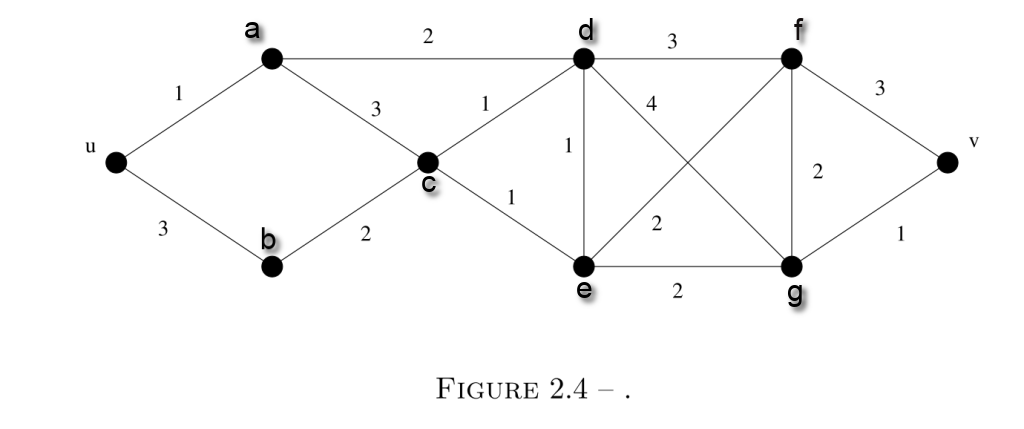
\includegraphics[width=1\columnwidth]{Figure2.4.png} % Example image
\end{center}
\subsection*{Réponse}
\begin{center}
l’algorithme de Dijkstra\\
	\begin{tabular}{l l l l l l l l l l}
		\toprule
		\textit{Sommet} & u & a & b & c & d &e & f & g & v\\
		\midrule
		Distance &  \textcolor{red}{0} & 1 &3 & $\infty$ & $\infty$  & $\infty$  & $\infty$  & $\infty$  & $\infty$  \\
		Distance &  \textcolor{red}{0} & \textcolor{red}{1} &3 & 4 & 3  & $\infty$  & $\infty$  & $\infty$  & $\infty$  \\
		Distance &  \textcolor{red}{0} & \textcolor{red}{1} &\textcolor{red}{3} & 4 & \textcolor{red}{3}  & 4  & 6  & 7  & $\infty$  \\
		Distance &  \textcolor{red}{0} & \textcolor{red}{1} &\textcolor{red}{3} & \textcolor{red}{4} & \textcolor{red}{3}  & \textcolor{red}{4}  & 6  & 6  & $\infty$  \\
		Distance &  \textcolor{red}{0} & \textcolor{red}{1} &\textcolor{red}{3} & \textcolor{red}{4} & \textcolor{red}{3}  & \textcolor{red}{4}  & \textcolor{red}{6}  & \textcolor{red}{6}  & 7  \\
		Distance &  \textcolor{red}{0} & \textcolor{red}{1} &\textcolor{red}{3} & \textcolor{red}{4} & \textcolor{red}{3}  & \textcolor{red}{4}  & \textcolor{red}{6}  & \textcolor{red}{6}  & \textcolor{red}{7}  \\
		\bottomrule
	\end{tabular}
\end{center}

\section*{Exercice 2.10}
\begin{problem}
A partir de l’algorithme de Dijkstra, construire un algorithme qui
détermine le diamètre de chaque composante connexe d’un graphe. Quelle en est la
complexité ?
\end{problem}
\subsection*{Réponse}

On fait l'algo Dijkstra pour tous les sommets  dans chaque composante connexe, retourner le plus grand nombre.

Complexity : n * algo Dijkstra ( on considere c'est $O(m + n log n)$  à l’aide de tas de Fibonacci) \\

Donc c'est $ O(n(m+n log n))$

\section*{Exercice 3.1.}
\begin{problem}
Les graphes de la figure 2.4 contiennent-ils un chemin eulérien, un cycle
eulérien, un chemin hamiltonien, un cycle hamiltonien ?
\end{problem}
\subsection*{Réponse}
\begin{center}
	\begin{tabular}{l l l l}
		\toprule
		\textit{} & G1 & G2 & G3 \\
		\midrule
		Chemin eulérien & true & true & false\\
		Cycle eulérien & false & true & false\\
		Chemin hamiltonien & true & false & true\\
		Cycle hamiltonien & true & false & false\\
		\bottomrule
	\end{tabular}
\end{center}

\section*{Exercice 3.2.}
\begin{problem}
Résoudre le problème du postier sur le graphe de la figure 3.2
\end{problem}

\begin{center}
	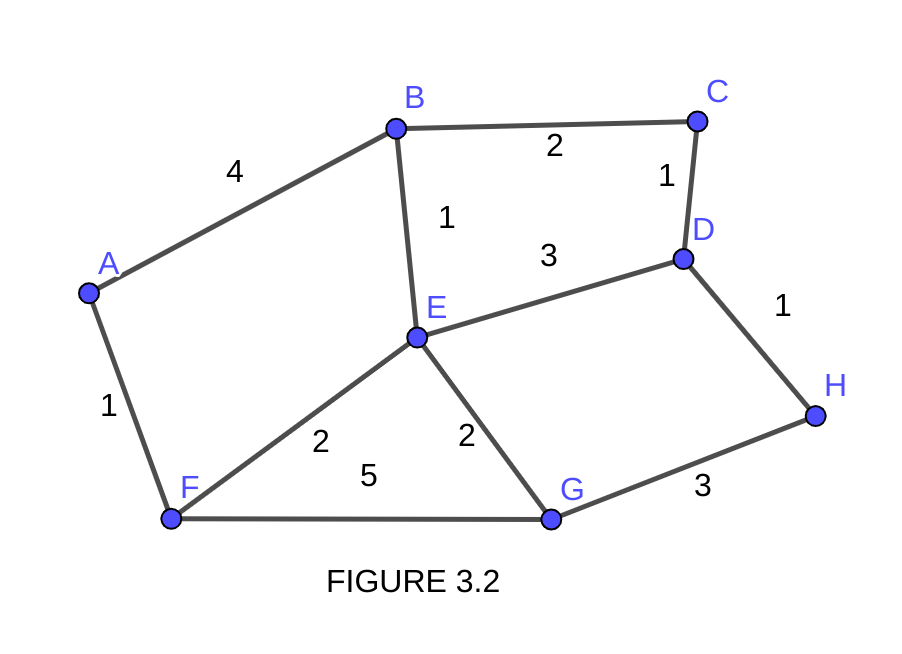
\includegraphics[width=0.5\columnwidth]{Figure3.2.png} % Example image
\end{center}

\subsection*{Réponse}Au premier, il faut trouver les sommets qui degre est impair. Donc on a sommet F, B, G, D. Ensuite on construire le Figure 3.2a\\

\begin{center}
	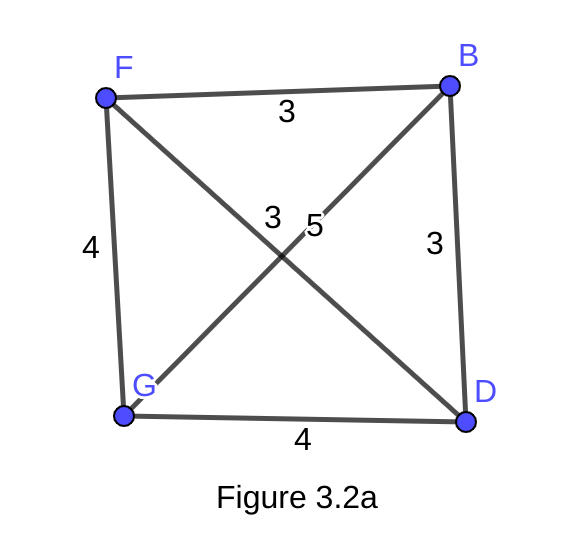
\includegraphics[width=0.5\columnwidth]{Figure3.2a.png} % Example image
\end{center}

Selon le Figure 3.2a, on veut connecter les 4 sommets avec le minimal poid, on peut choisir Edge(F, G) et Edge(B, D).\\

On peut ajouter un Edge(B, D) dans le Figure 3.2, donc il y a seulement 2 sommets impaire, on peut trouver un chemin eulerien.\\

Le poids minimal total est l'addition de tous les poids de Figure3.2 et Edge(F,G), Edge(B,D).\\

Tous les poids de Figure3.2 : \(1+4+2+1+1+3+2+2+5+1+3 = 25\)\\
Avec les 2 autre edges : \(25 + 3 + 4 = 32\)\\

Donc le poids minimal total est \textbf{32}.

\newpage
\part*{Partie codes}

\section*{TP6.B. Visualisation de Graphes}
\subsection*{JGraphT}
Je utilise le bibliotheque JGraphT pour visualiser graphe. Une partie de mon code d'affichage.

\lstinputlisting[
		caption=GrapheGenerate, % Caption above the listing
		label=lst:luftballons, % Label for referencing this listing
		language=Java, % Use Perl functions/syntax highlighting
		frame=single, % Frame around the code listing
		showstringspaces=false, % Don't put marks in string spaces
		numbers=left, % Line numbers on left
		numberstyle=\tiny, % Line numbers styling
	]{GraphGenerate.java}

\newpage

Voici le resultat du code:\\
\begin{center}
	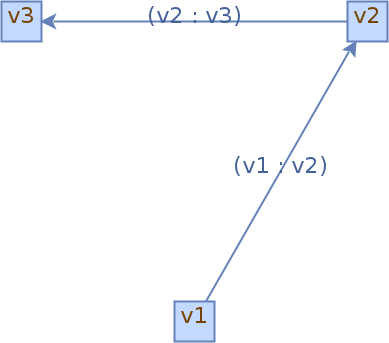
\includegraphics[width=0.6\columnwidth]{graph.png} % Example image
\end{center}

\subsection*{Neo4j}
Neo4j est une base de données non relationnelle, une base de données graphique native. Dans une base de données relationnelle normale, la recherche d'un élément de données nécessite souvent l'interrogation de plusieurs tables de la base de données, en particulier pour les grands projets qui nécessitent de nombreuses et longues requêtes sautantes. Les performances de ce type de base de données sont réduites dans ce scénario. La base de données de graphes introduit le concept de Edge entre les Vertex, ce qui améliore considérablement les performances dans ce scénario.\\

\textbf{Neo4j Java}
\lstinputlisting[
		caption=Neo4j avec Java exemple, % Caption above the listing
		label=lst:luftballons, % Label for referencing this listing
		language=Java, % Use Perl functions/syntax highlighting
		frame=single, % Frame around the code listing
		showstringspaces=false, % Don't put marks in string spaces
		numbers=left, % Line numbers on left
		numberstyle=\tiny, % Line numbers styling
	]{NeoJava.java}
Voici le resultat dans le terminale:\\
Node1 relation12 Node2

\newpage
\textbf{Neo4j browser}
Neo4j browser est un interface graphique pour modifier les datas de database. Il utilise Cypher au lieu de SQL language. \\
 \\
Create record:
\begin{center}
	CREATE (Letao:Person {name:'Letao WANG', born:1999})
\end{center}




\begin{lstlisting}
	CREATE (UniversityOfParis:University 
	{title:'University of Paris', released:2019, 
		tagline:'Welcome to the University of Paris'})
	CREATE (Taole:Person {name:'Taole WANG', born:1999})
	CREATE (Stan:Person {name:'Stan Ma', born:1999})
	CREATE (Paul:Person {name:'Paul Hu', born:1999})
	
	CREATE (Taole)-[:STUDIED_IN {roles:['Student']}]->
	(UniversityOfParis)
\end{lstlisting}

Query:
\begin{center}
	MATCH (Letao:Person {name: "Letao WANG"}) RETURN Letao\\ 
	
	
	
\end{center}

\begin{center}
	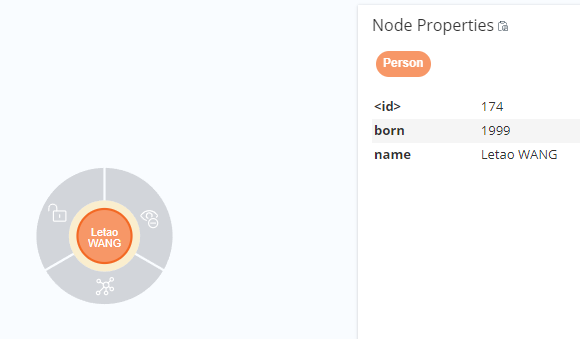
\includegraphics[width=0.5\columnwidth]{NeoWang.png} % Example image
	\newline\newline
	Et on peut identifier la relation entre Person et University aussi, par exemple on cherche les personnes qui etudier a Universite de Paris\newline\newline
	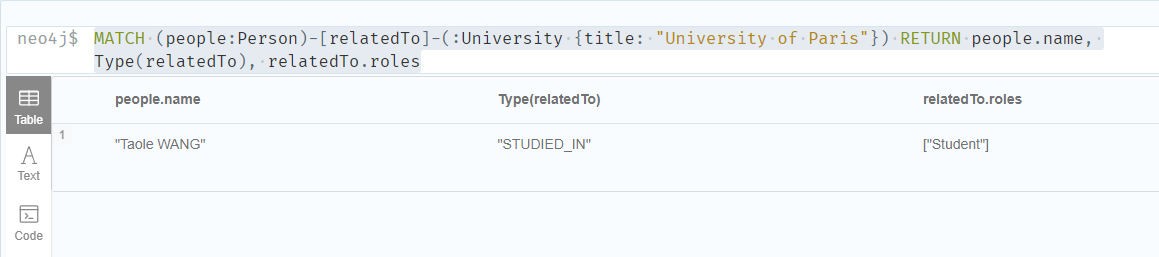
\includegraphics[width=1\columnwidth]{NeoUParis.png} % Example image
\end{center}

\newpage
\section*{TP7 PartieB}
\subsection*{Algo Dijkstra}
Apres j'ai telecharge les fichiers, j'ai realise que le projet est ecrire par Java, mais le style est tres comme language C. Donc au premier je reformule un peu la structure du projet, un peu plus comme MVC (Bien sur je vais continuer le modifier).\\
\begin{center}
	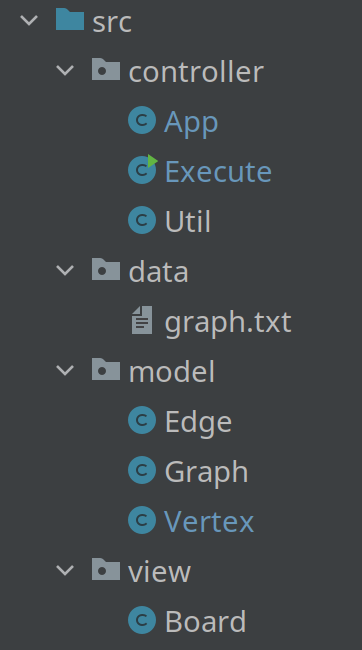
\includegraphics[width=0.3\columnwidth]{structure_v1.0.png}
\end{center}
Aussi encapsulation, c'est a dire ajouter "pivate" avant les attributs\\

\textbf{Certaines methodes importants}\\
\newline
Get Neighbors
\begin{lstlisting}
     /**
     * For getting all max to 8 neighbors of this vertex
     * @param line line of source
     * @param col col of source
     * @param nlines number of lines
     * @param ncols number of cols
     * @return list of neighbors vertex
     */
    public static ArrayList<Integer> getNeighborDest
	(int line, int col, int nlines, int ncols) 
\end{lstlisting}
\newpage
Set weights of Edges
\begin{lstlisting}
	/* direction horizontally or vertically */
	if (Math.abs(source - dest) == 1 || 
		Math.abs(source - dest) == ncols) {
		weight = (timeDest + timeSrc) / 2;
	}
	/*  direction  diagonal */
	double weight12 = Math.sqrt(Math.pow(weight1, 2) 
	+ Math.pow(weight2, 2));

	double weight34 = Math.sqrt(Math.pow(weight3, 2)
	 + Math.pow(weight4, 2));

	weight = Math.min(weight12, weight34);
\end{lstlisting}

Partie de algo Dijkstra
\begin{lstlisting}
	/* pour tous ses voisins, on verifie si 
		on est plus rapide en passant par ce noeud. */
        for (int i = 0; i < graph.getVertexlist().get(min_v).
			getAdjacencylist().size(); i++) {
        		int to_try = 
		graph.getVertexlist().get(min_v).
		getAdjacencylist().get(i).getDestination();

                /* to_try node timeFromSource += weight */
                /* code etc. */
        }
\end{lstlisting}

\newpage
\textbf{Resultat}\\
Parce que la partie graphe de projet est deja fini, je n'ai pas besoin d'ecrire les interface graphique.\\
\begin{center}
	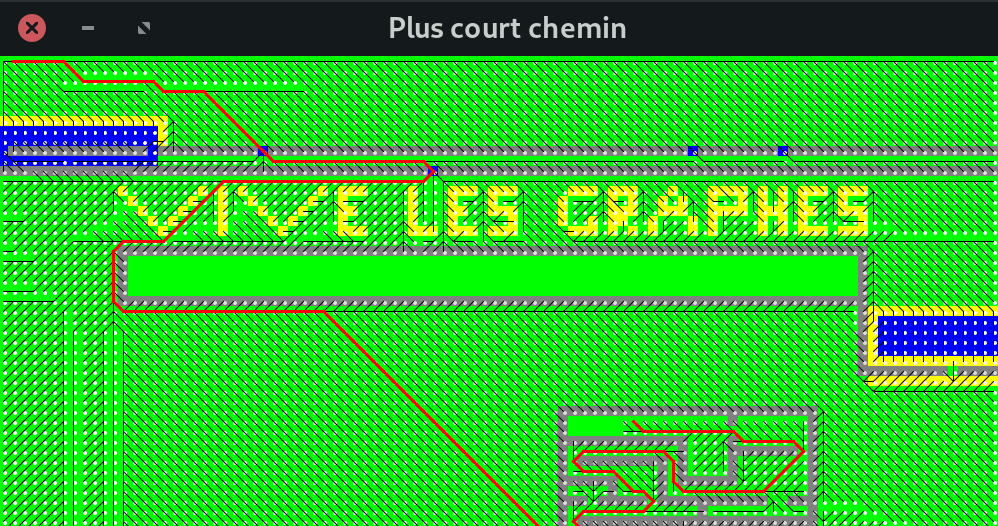
\includegraphics[width=1\columnwidth]{TP7B_dijkstra.png}
\end{center}
les lines noir sont des Edges, et le line rouge est le chemin minimal distance entre Vertex start a Vertex end.

\begin{center}
	Et dans le terminale
	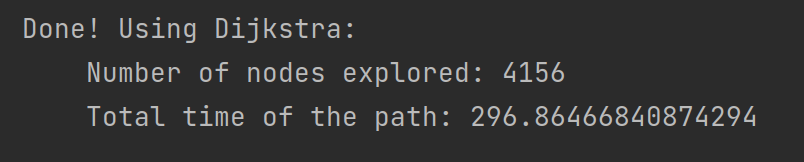
\includegraphics[width=1\columnwidth]{TD7B_dijkstra_res.png}
\end{center}

Partie Algo Dijkstra fini.
\end{document}
